\documentclass[11pt]{standalone}
\usepackage{amssymb}
\usepackage{amsmath}
\usepackage[no-math]{fontspec}
\usepackage{unicode-math}
\usepackage{libertinus}
\usepackage{pgf,xcolor}
\usepackage{tikz}
\usetikzlibrary{arrows.meta, backgrounds}
\usepackage{pgfplots}
\pgfplotsset{compat=newest}

\definecolor{my_darkgray}{HTML}{484949}
\definecolor{my_lightgray}{HTML}{F3F4F4}
\definecolor{my_darkblue}{HTML}{005A94}
\definecolor{my_lightblue}{HTML}{CCDEE9}
\definecolor{my_yellow}{HTML}{FFEC7F}
\definecolor{my_red}{HTML}{E60000}
\definecolor{my_orange}{HTML}{E87846}

\begin{document}
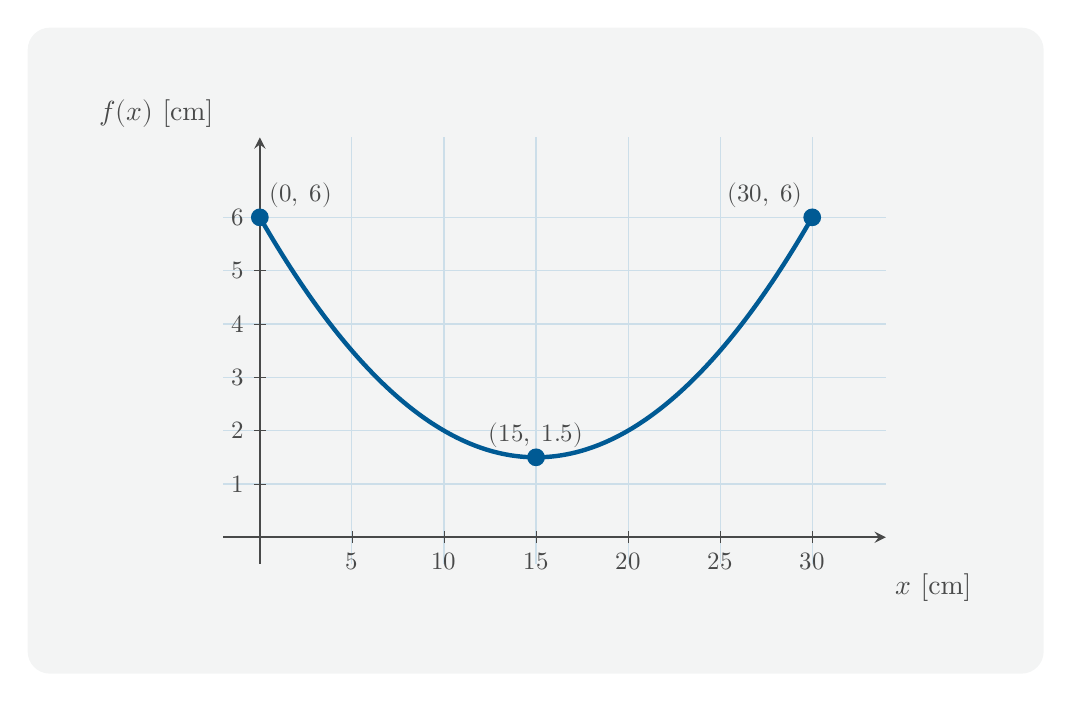
\begin{tikzpicture}[
    show background rectangle,
    background rectangle/.style={fill=my_lightgray, rounded corners=8pt},
    inner frame sep=0.8cm
]
  \begin{axis}[
    % axis equal omitted: x-domain spans 30 units, y-domain ~5 units;
    % equal scaling would produce an unreadably wide figure.
    width  = 10cm,
    height = 7cm,
    axis lines      = center,
    axis line style = {thick, my_darkgray},
    xlabel          = {$x$ [cm]},
    ylabel          = {$f(x)$ [cm]},
    xlabel style    = {color=my_darkgray, at={(axis description cs:1,0)},
                       anchor=north west},
    ylabel style    = {color=my_darkgray, at={(axis description cs:0,1)},
                       anchor=south east},
    xmin = -2,  xmax = 34,
    ymin = -0.5, ymax = 7.5,
    xtick      = {0, 5, 10, 15, 20, 25, 30},
    ytick      = {0, 1, 2, 3, 4, 5, 6},
    tick style = {color=my_darkgray},
    tick label style = {color=my_darkgray, font=\small},
    grid            = both,
    grid style      = {color=my_lightblue, thin},
    major grid style= {color=my_lightblue},
  ]

    %% Parabolic marble track f(x) = 0.02x^2 - 0.6x + 6
    \addplot[
      draw    = my_darkblue,
      samples = 300,
      ultra thick,
      domain  = 0:30,
    ]{ 0.02*x^2 - 0.6*x + 6 };

    %% Vertex at (15, 1.5)
    \addplot[
      only marks,
      mark        = *,
      mark size   = 3pt,
      draw        = my_darkblue,
      fill        = my_darkblue,
    ] coordinates { (15, 1.5) };
    \node[color=my_darkgray, above, font=\small]
      at (axis cs:15, 1.5) {$(15,\;1.5)$};

    %% Start point (0, 6)
    \addplot[
      only marks,
      mark        = *,
      mark size   = 3pt,
      draw        = my_darkblue,
      fill        = my_darkblue,
    ] coordinates { (0, 6) };
    \node[color=my_darkgray, above right, font=\small]
      at (axis cs:0, 6) {$(0,\;6)$};

    %% End point (30, 6)
    \addplot[
      only marks,
      mark        = *,
      mark size   = 3pt,
      draw        = my_darkblue,
      fill        = my_darkblue,
    ] coordinates { (30, 6) };
    \node[color=my_darkgray, above left, font=\small]
      at (axis cs:30, 6) {$(30,\;6)$};

  \end{axis}
\end{tikzpicture}
\end{document}
